\chapter{Interferometry, Calibration \& Polarimetry}
\label{chapter:interferometry}

In this Chapter I wished to build a formalism around wide-field, polarized interferometric measurements that could be used throughout this work. Many traditional assumptions used in radio interferometry are broken in the case of the wide-field, fully-polarized, drift-scanning measurements native to interferometric EoR observations. In Section~\ref{sec:interferometry_vis}, I derive the equation describing the fundamental observable for an interferometer, called a ``visibility". Section~\ref{sec:interferometry_cal}, I describe calibration techniques relevant to this work and in Section~\ref{sec:interferometry_pol} I review some of the implications of the previous two sections for polarized measurements.

For a comprehensive review of interferometry from a more traditional perspective, see \cite{TMS}.

\section{The Visibility Equation}
\label{sec:interferometry_vis}

A radio interferometer (a term used interchangeably with ``interferometric array" for radio observations) is an ensemble of receiving elements, where each element's measurement is correlated with every other element's. The simplest case is a two-element interferometer, which we will focus on below. We assume that the elements are coplanar and identical.

\subsection{The Classical Visibility Equation}

Consider two receiving elements $i$ and $j$, separated by baseline vector $\vec{b}$. Suppose a plane wave of wavelength $\lambda$ is incident upon these elements, with direction of propagation $-\hat{s}$. The geometry of this interferometer is illustrated in Figure~\ref{fig:interferometry_2element}.

\begin{figure}
\centering
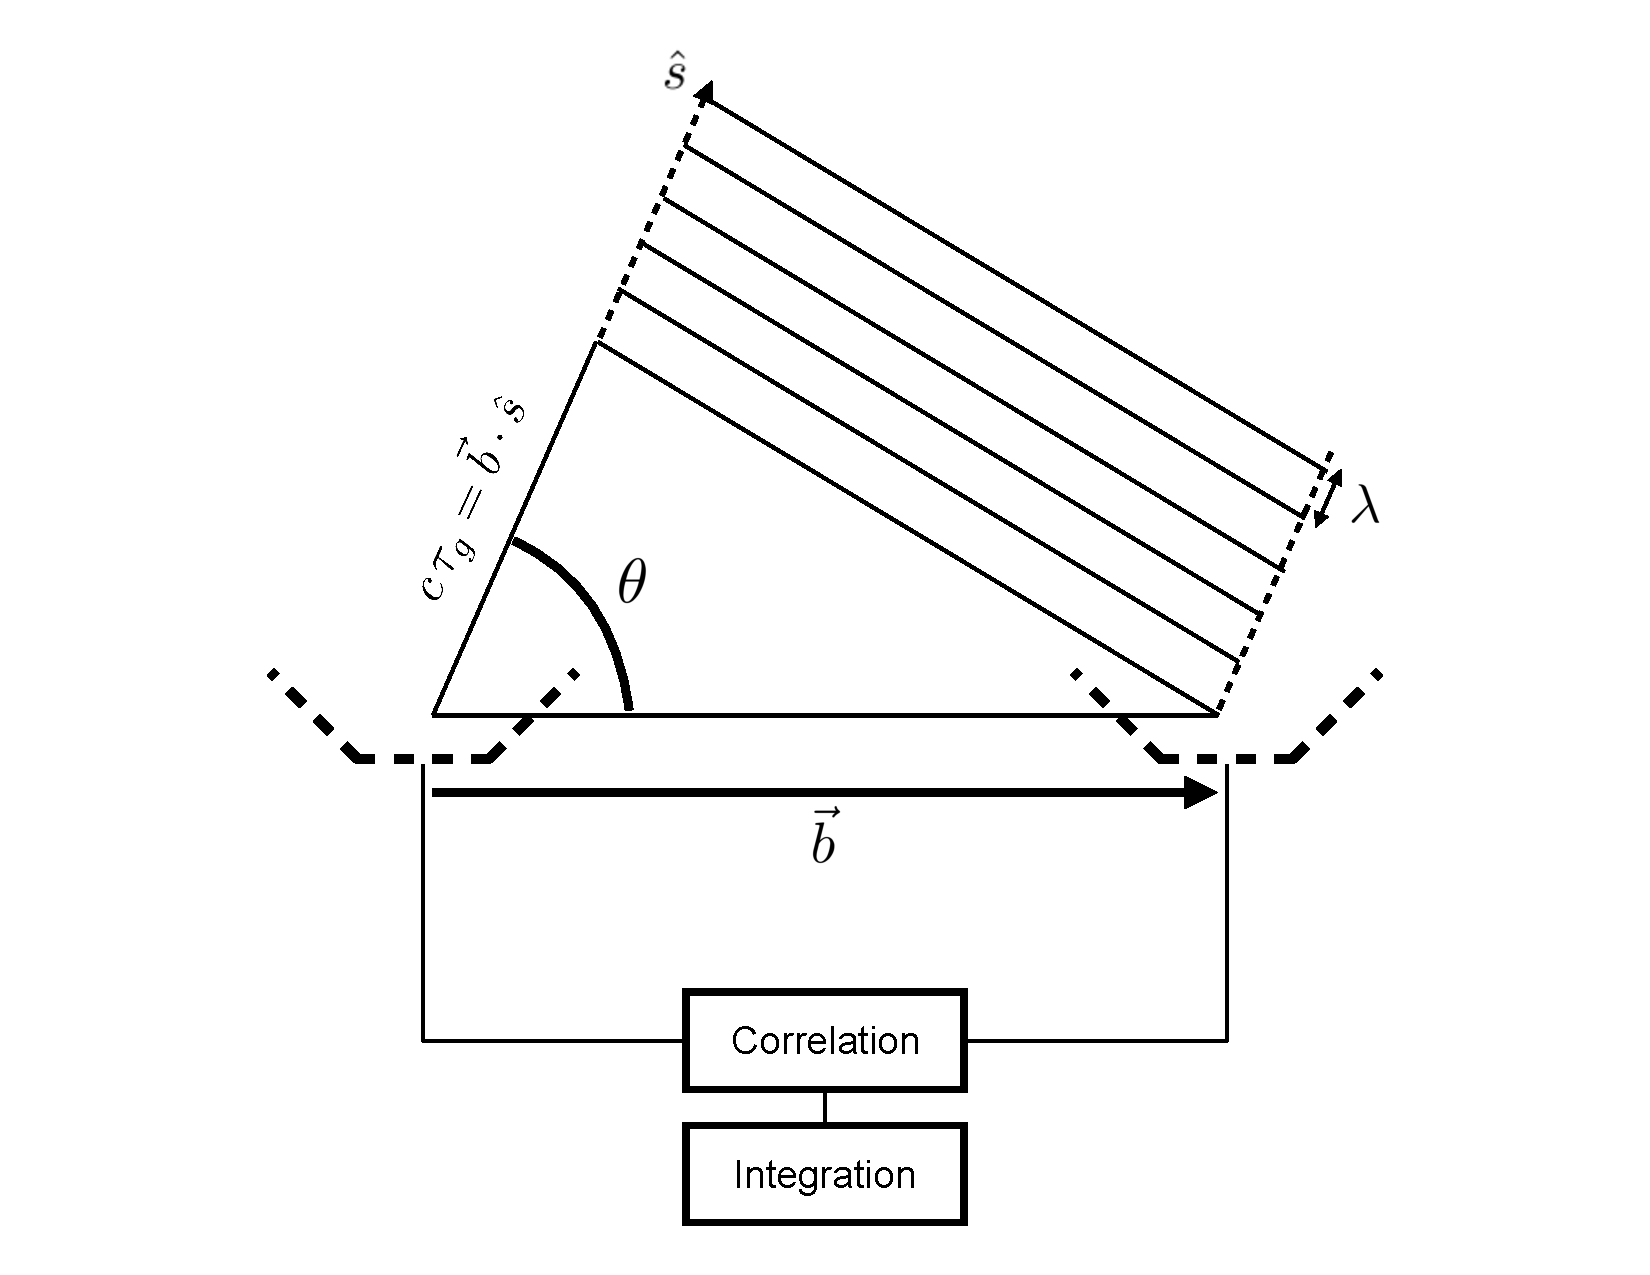
\includegraphics[width=0.9\textwidth]{chapters/interferometry/figures/visibility_explanation.pdf}
\caption{The geometry of a two-element interferometer, with a plane wave incident from direction $\hat{s}$.}
\label{fig:interferometry_2element}
\end{figure}

We can define the electromagnetic wave to have a frequency dependent phase, such that the electric field measured by element $i$ at time $t$ is

\begin{equation}
E_i = E_0 e^{-2\pi i \nu t}.
\label{eq:Ei}
\end{equation}

The time difference between the arrival at $i$ and $j$ is called the ``geometrical delay", $\tau_g$:

\begin{equation}
\tau_g = \frac{\vec{b}\cdot\hat{s}}{c},
\end{equation}
and the electric field measured by element $j$ is

\begin{equation}
E_j = E_0 e^{-2\pi i \nu (t+\tau_g)}.
\end{equation}

An interferometer is an instrument which measured voltages induced by these electric fields, and correlates them together, integrating their product over some coherent time-scale. This correlation grants:

\begin{equation}
\langle E_i E_j^* \rangle 
= \lim_{T\rightarrow\inf}\frac{1}{2T}\int^T_{-T} E_i(t) E_j(t) {\rm d}t
= | E_0 |^2 e^{-2\pi i \nu \tau_g}
\label{eq:vis_time_integration}
\end{equation}
where $e^{-2\pi i \nu \tau_g} = e^{-2\pi i \nu \vec{b}_{ij}\cdot\hat{s}/c}$ is known as the ``fringe" term, due to its sinusoidal nature. We can generalize this relationship to include more than a single plane wave from direction $\hat{s}$. Many plane waves, from all directions, can be incident upon the interferometer at a given time and frequency. We can represent the power distribution on the sky as $S(\Omega)$, where $S(\Omega)$. However, no instrument is equally sensitive to radiation from every direction $\hat{s} \in \Omega$. Instead, an instrument has some sensitivity pattern -- a \textit{beam pattern} -- that tapers the power distribution on the sky into an ``observed sky",  $S'(\Omega) = A(\Omega)S(\Omega)$. 

These generalizations lead to the classical visibility equation:

\begin{equation}
V_{ij}(\nu) = \int A(\Omega, \nu) S(\Omega, \nu) e^{-2\pi i \nu \vec{b}_{ij}\cdot\hat{s}/c} {\rm d}\Omega
\label{eq:classical_visibility}
\end{equation}
for a ``visibility" -- the fundamental interferometric observable -- $V_{ij}$ as a function of frequency.

If we choose to represent the source direction in terms of directional cosines $\ell$ and $m$, and represent the baseline vector in units of wavelengths, $\vec{b}_{ij}/\lambda=(u,v,w)$, we can perform a change of variables in Equation~\ref{eq:classical_visibility} to give

\begin{equation}
V_{ij}(u,v) = \int\int A(\ell, m)S(\ell, m) e^{-2\pi i (u\ell + vm + w\sqrt{1 - \ell^2 - m^2})} \frac{ {\rm d}\ell {\rm d}m }{\sqrt{1 - \ell^2 - m^2}}.
\label{eq:vis_def_widefield}
\end{equation}

This relationship is often simplified by assuming only a small area of the sky is under observation -- that is, that $A(\ell,m)$ falls-off steeply from zenith -- and therefore $\ell^2$ and $m^2$ are small. This grants

\begin{equation}
V_{ij}(u,v) \approx e^{-2\pi i w} \int\int A(\ell, m)S(\ell, m) e^{-2\pi i (u\ell + vm)} {\rm d}\ell {\rm d}m,
\label{eq:vis_dev_narrowfield}
\end{equation}
which plainly casts $V(u,v)$ as the Fourier transform of the observed sky if $w$ is small: that is, the array is co-planar and no appreciable curvature of the sky is probed. Modern low frequency interferometers used in this work greatly violate this approximation, the consequences of which I will discuss in the proceeding sections.

Even though it is often violated, the Fourier relationship shown in Equation~\ref{eq:vis_dev_narrowfield} is an extremely useful one to work with when translating between visibilities and images. Images can be created by inverse Fourier transforming all of the visibilities measured by an array. Following Equation~\ref{eq:vis_def_widefield}, a reconstructed image $\tilde{S}(\ell, m)$ is given by

\begin{equation}
\frac{A(\ell, m)\tilde{S}(\ell, m)}{\sqrt{1 - \ell^2 - m^2}} = \int\int \Xi(u, v) V(u,v) e^{2\pi i \nu (u\ell + vm)} {\rm d}u {\rm d}v.
\label{eq:image_estimate}
\end{equation}

In Equation~\ref{eq:image_estimate}, we see that the reconstructed image $\tilde{S}(\ell, m)$ is attenuated by the beam response $A(\ell, m)/\sqrt{1 - \ell^2 - m^2}$. The function $\Xi(u, v)$ defines the sampling of the $u,\,v$ - plane. It is equal to 1 at the points sampled by the interferometer (baselines of length and direction defined by the vector  $\vec{b} = (u,v)$ exist in the array) and 0 elsewhere. As an example, the ``array" shown in Figure~\ref{fig:interferometry_2element} would be described by a $\Xi(u, v)$ function that was zero at all points except for a single ($u,\,v$) coordinate described by baseline vector $\vec{b}$.

The effect of the sampling function $\Xi(u, v)$ is that the true sky $S(\ell,m)$ can never be completely reconstructed, since it is impossible to build an interferometer that samples every $u,v$ mode. The true sky is convolved with the Fourier transform of $\Xi(u, v)$, which astronomers refer to as the ``dirty beam". $\Xi(u, v)$ contains zeros, so a complete deconvolution of $\tilde{S}(\ell, m)$ is impossible.

We now note that an important aspect of light has been absent throughout the derivations above: the polarization state of the radio wave that induces the electric field in Equation~\ref{eq:Ei}. Interferometers are typically constructed with two feeds, sensitive to polarization states of an incident radio wave along two separate axes. In the case of all of the instruments used in this work (see Chapter~\ref{chapter:instruments}), an antenna $i$ had two dipole feeds perpendicular to one another. These were along the North-South direction (`n') and the East-West direction (`e'). We can attempt to generalize Equation~\ref{eq:classical_visibility} to include polarization, setting antenna $i$ to have orientation $p$ and antenna $j$ to have orientation $q$, $p,q\in(e,n)$:

\begin{equation}
V^{pq}_{ij} = \int A_{pq}(\Omega, \nu) S_{pq}(\Omega, \nu) e^{-2\pi i \nu \vec{b}_{ij}\cdot\hat{s}/c} {\rm d}\Omega.
\end{equation} 
However, two aspects of this equation are unsatisfactory. As explored in Chapter~\ref{chapter:astro_rad}, the polarized sky is defined with the four Stokes parameters; an ``$S_{pq}$" polarized sky does not exist. Likewise, a dipole is not purely sensitive to a single vector orientation from the sky, but probes a wide range of angles\footnote{In the case of the PAPER instrument, described in the next Chapter, the dipole feeds probed the entire hemisphere of the sky.}. Therefore a $A_{pq}$ polarized beam is ill-defined. These shortcomings lead us to rewrite the visibility equation, cohesively including polarization from the outset.  

\subsection{The Measurement Equation}

The Radio Interferometric Measurement Equation (RIME) provides an extremely useful framework for describing wide-field polarized observations. Formulated by \cite{HBS.1.96}, it was re-introduced to the radio astronomy community through a series of papers by O.~M. Smirnov \citep{Smirnov.11, Smirnov.11.2, Smirnov.11.3, Smirnov.11.4}. In this section I review the portions of his work most relevant to this thesis, and defer the reader to the series for a useful and thorough walk-through of wide-field radio interferometry and high dynamic-range calibration.

Returning to Equation~\ref{eq:Ei}, a radio wave incident on an antenna induces a voltage in along feed arm

\begin{equation}
\vec{E} = (e_p, e_q);\,\,\,\vec{v} = (v_p,v_q) = \textbf{J}\vec{E}
\label{eq:voltage_jones}
\end{equation}
where \textbf{J} is a $2\times2$ complex matrix termed the ``Jones matrix" \citep{Jones.41}. Jones matrices represent linear transformations along the signal path, from the emission of the radio wave onwards. Multiple stages along the signal propagation can be represented by multiplying different Jones matrices together as a ``Jones chain", which may be expanded or collapsed as convenient.

Interferometric visibilities are pairwise correlations of the components of $\vec{v}$ between antennas $i$ and $j$, integrated over some small time span (Equation~\ref{eq:vis_time_integration}), which we can represent hold in matrix form (the layout of which will become clear in a moment):

\begin{equation}
\textbf{V}_{ij} = \begin{pmatrix} 
\langle v^p_i v^{p*}_j \rangle & \langle v^p_i v^{q*}_j \rangle \\
\langle v^q_i v^{p*}_j \rangle & \langle v^q_i v^{q*}_j \rangle \\
 \end{pmatrix} = \langle \vec{v}_i \vec{v}^H_j \rangle.
\end{equation}
Above, H represents the Hermitian transpose operation.

Using this formalism allows us to map the emitted electric field to the observed visibilities, 
\begin{equation}
\textbf{V}_{ij} = \textbf{J}_i \begin{pmatrix} 
\langle e^p_i e^{p*}_j \rangle & \langle e^p_i e^{q*}_j \rangle \\
\langle e^q_i e^{p*}_j \rangle & \langle e^q_i e^{q*}_j \rangle \\
 \end{pmatrix} \textbf{J}^H_j = \textbf{J}_i \textbf{C}_{ij} \textbf{J}^H_j
\end{equation}
where \textbf{J}$_{i,j}$ may be Jones chains of arbitrary length. We have assumed instrument stability to move them out of the time averages in the central matrix. We refer to $\textbf{C}_{ij}$ as the ``coherency matrix". 

In Chapter~\ref{chapter:astro_rad} the Stokes parameters we introduced. \cite{Hamaker-Bregman.96} showed that the components of the coherency matrix are closely related to the Stokes parameters:

\begin{equation}
\begin{pmatrix} 
\langle e^p_i e^{p*}_j \rangle & \langle e^p_i e^{q*}_j \rangle \\
\langle e^q_i e^{p*}_j \rangle & \langle e^q_i e^{q*}_j \rangle \\
 \end{pmatrix}
 =
 \begin{pmatrix} 
I + Q & U + iV \\
U - iV & I - Q \\
 \end{pmatrix}.
 \label{eq:interferometry-stokes-coherency}
\end{equation}

The Jones formalism allows for a construction of the visibility equation that does not make explicit assumptions regarding polarization or field-of-view, in which we can map the Stokes parameters into the instrumental basis that visibilities are computed in:

\begin{equation}
\textbf{V}_{ij} = \int \textbf{J}_i(\hat{s}) \textbf{C}_{ij}(\hat{s}) \textbf{J}_j^H(\hat{s}) e^{-2\pi i \nu \vec{b}_{ij}\cdot\hat{s}/c} {\rm d}\Omega,
\label{eq:RIME}
\end{equation}
which \cite{Smirnov.11} refers to as the ``Full Sky Radio Interferometric Measurement Equation"\footnote{We choose to explicitly show the exponent in this formulation for ease of comparison with Equation~\ref{eq:classical_visibility}. \cite{Smirnov.11} shows that this term can written as a ``phase delay Jones matrix" and absorbed into the Jones chain.}. Note that all of these quantities are functions of frequency as well, in general.

So far, the formalism shown has used the $2\times 2$ ``Jones basis". It is sometimes more useful to work in the $4\times 4$ ``Mueller basis" \citep{Mueller.48}, which acts on visibilities in $4\times 1$ vector form:

\begin{equation}
\begin{pmatrix}
V^I \\
V^Q \\
V^U \\
V^V \\
\end{pmatrix}
=
\textbf{S}\vec{V}_{ij}
= 
\begin{pmatrix}
1 & 0 & 0 & 1 \\
-1 & 0 & 0 & 1\\
0 & 1 & 1 & 0 \\
0 & -i & i & 0 \\
\end{pmatrix}
\begin{pmatrix}
V^{pp} \\
V^{pq} \\
V^{qp} \\
V^{qq} \\
\end{pmatrix}.
\label{eq:interferometry_pseudo_stokes}
\end{equation} 

It is important to note that Equation~\ref{eq:interferometry_pseudo_stokes} lists a vector of ``Stokes-polarized visibilities" on the left-hand side, whereas  Equation~\ref{eq:interferometry-stokes-coherency} shows that the coherency matrix contains linear combinations the Stokes parameters. This is not an inconsistency. While visibilities are quantities that are integrated over the sky, the Stokes parameters are only defined \textit{on} the sky. One must transform the visibilities from the $uv$-plane onto the image-plane and deconvolve the beam in order to measure the Stokes parameters. Instead, linear combinations of visibilities measure a proxy for each the Stokes parameters. To make the inequality between visibilities and Stokes parameters explicit, I will refer to the ``Stokes-polarized visibilities" as ``pseudo-Stokes visibilities" from now on.

One can translate between these two formalisms using the definition of $\vec{V}_{ij}$ (c.f. Equation~\ref{eq:voltage_jones}),

\begin{equation}
\vec{V}_{ij} = (\textbf{J}_i \otimes \textbf{J}_j^H)(\vec{E}\otimes\vec{E}^H).
\end{equation}

Comparison of Equation~\ref{eq:classical_visibility} and \ref{eq:RIME} shows that the Jones chain must, at the very least, encapsulate the beam pattern of the instrument. We can build such a Jones matrix by considering the response of feed $p$ on antenna $i$ to an electric field from infinity in the direction ($\theta$, $\phi$):

\begin{equation}
\vec{A}_i^p(\hat{s}) = A^p_{i,\theta}(\hat{s})\hat{\theta} + A^p_{i,\phi}(\hat{s})\hat{\phi},
\end{equation}
where we have suppressed the frequency dependence. The antenna patterns may be written as components of a ``Beam Jones matrix" for an antenna,

\begin{equation}
\textbf{J}_i^{\rm B}(\hat{s}) = 
\begin{pmatrix}
A^p_{i,\theta}(\hat{s}) & A^p_{i,\phi}(\hat{s}) \\
A^q_{i,\theta}(\hat{s}) & A^q_{i,\phi}(\hat{s}) \\
\end{pmatrix}.
\label{eq:jones-beam}
\end{equation}

These are the essential components for understanding the fundamental measurement performed by an interferometer. However, there are several effects one must take into account for the equations to truly reflect an interferometric measurement; effects such as instrumental gains, reflections between antennas, Faraday rotation in the ionosphere, etc. Most importantly, we must consider how these factors affect the measurement of polarization.

\section{Calibration Techniques}
\label{sec:interferometry_cal}

The purpose of calibration is to remove effects of the instrument and the atmosphere from the data. Visibilities are measured in ``data units". That is, a given feed on an antenna will record some measurement of power, but some scalar conversion factor is required to calibrate that power to units of flux density. As visibilities measure the pairwise correlations of antenna powers, the estimation of the calibration factors can quickly become difficult as the number of antennas increases. In this Section we explain different approaches to such a challenge.

\subsection{Diagonal and off-diagonal calibration}

The calibration term that converts the power measured by an antenna to physical units is referred to as the ``antenna gain". This may be summarized per feed as a direction-independent ``Gain Jones matrix",

\begin{equation}
\textbf{J}_i^{\rm G} = 
\begin{pmatrix}
g_i^p &0 \\
0 & g_i^q\\
\end{pmatrix},
\label{eq:jones-gains}
\end{equation}
where we have suppressed the frequency dependence. The components of $\textbf{J}_i^{\rm G}$ are complex numbers, the argument of which represents instrumental phase, and the modulus represents instrumental amplitude. Note that this formulation of $\textbf{J}_i^{\rm G}$ is only appropriate for linear antenna feeds. Circular feeds, which we will not comment on for the rest of this work, require an additional rotation matrix applied to move from a linear to a circular polarization frame.

Unfortunately, a direction-independent scaling is not the only term that requires estimation. As Equation~\ref{eq:jones-beam} makes clear, a given feed is not receptive to a single plane of polarization. In general, we expect some fraction of power measured by feed $p$ to be transferred into feed $q$ via imperfect electronics \citep[clever feed designs can attempt to minimize this effect, e.g.][]{Parashare.06, Parsons.10}. This kind of power leakage is described by an off-diagonal matrix, and the components are known as ``\textit{D}-terms",

\begin{equation}
\textbf{J}_i^{\rm D} = 
\begin{pmatrix}
1 & D_i^p \\
D_i^q & 1\\
\end{pmatrix}.
\end{equation}

\textit{D}-terms are often left un-calibrated, as they are generally a few percent of the gain term for a given feed. However, a $\sim$5\% error in calibration could represent an error large enough to inhibit an EoR detection. Unless an EoR instrument is shown to have very low D-terms, they must be taken in to account.

\subsubsection{Ionospheric effects}

Chapter~\ref{chapter:ionosphere} details the importance of the ionosphere for EoR measurements. Briefly put, the ionosphere is an upper layer of the Earth's atmosphere; an ionized plasma formed from solar radiation. Coupled with the Earth's magnetic field, it becomes a time- and position-variable Faraday screen (see Chapter~\ref{chapter:astro_rad}) capable of rotating the polarization axis of an incident electromagnetic wave. This adds an additional term to the Jones chain in Equation~\ref{eq:RIME}. Representing the ionospheric Faraday screen as $\Phi (\hat{s},t)$, this term is

\begin{equation}
\textbf{J}_i^{\rm I} = 
\begin{pmatrix}
\cos(2\Phi(\hat{s},t)c^2/\nu^2) & \sin(2\Phi(\hat{s},t)c^2/\nu^2) \\
-\sin(2\Phi(\hat{s},t)c^2/\nu^2) & \cos(2\Phi(\hat{s},t)c^2/\nu^2)\\
\end{pmatrix}.
\end{equation}

The ionosphere's effect on polarized radiation is the most important one to consider for this work. However, the more commonly worried-about effect of the ionosphere (among radio astronomers) is its diffractive property. Neglecting the Earth's magnetic field, the refractive index $\eta$ of a cold, collisionless plasma is \citep{TMS}

\begin{equation}
\eta = \sqrt{1 - \frac{\nu^2}{\nu_P^2}},
\label{eq:diffractive_ionosphere}
\end{equation}
for an electromagnetic wave of frequency $\nu$ and plasma frequency $\nu_P$, given by

\begin{equation}
\nu_P = \frac{1}{2\pi}\sqrt{\frac{n_e e^2}{m_e\epsilon_0}}
\end{equation}
where $n_e$ is the number density of electrons, $e$ and $m_e$ are the electron charge and mass and $\epsilon_0$ is the permittivity of free space. This term is typically of the order of a few MHz \citep{Vedantham.15}. This causes a direction- and time-dependent phase shift in the propagating wave. This shift is 

\begin{equation}
\gamma(\hat{s},\nu) = \int {\rm d}l \frac{2\pi\nu}{c}\eta(\hat{s}) \approx \int {\rm d}l \frac{2\pi\nu}{c} - \frac{1}{2}\int {\rm d}l \frac{2\pi\nu_P^2}{c\nu}
\end{equation}
where $l$ is the distance through the ionosphere, and we have Taylor-expanded Equation~\ref{eq:diffractive_ionosphere} for the approximation. This effect can be represented as a diagonal, direction-dependent Jones matrix,

\begin{equation}
\textbf{J}_i^{\rm \Gamma}(\hat{s},\nu) = 
\begin{pmatrix}
\exp(i\gamma(\hat{s},\nu)) &0 \\
0 & \exp(i\gamma(\hat{s},\nu))\\
\end{pmatrix},
\end{equation}
where we have made the frequency dependence explicit.

Due to the turbulent nature of the ionosphere, both of these terms are extremely difficult to calibrate \citep{Intema.09, Vedantham.15}. In Chapter~\ref{chapter:ionosphere}, we present the effects \textit{not} calibrating the polarized component when averaging together large numbers of polarized visibilities.

\subsection{Image-based calibration}

Traditionally, the approach taken for estimating the components of all of the above was to observe a calibration source. A calibrator source would be unresolved, such that its position and phase is a direct measure of ionospheric diffraction and instrumental phase. Deviation from its catalogued position can be subtracted off, calibrating the phase (the argument of the components of $\textbf{J}_i^{\rm G}$; Equation~\ref{eq:jones-gains}). For an interferometer that cannot point in a given direction, but instead ``drift-scans", observing the sky as the Earth rotates, calibration takes place when the calibrator source is at zenith (for a telescope that can point, the calibrator source would be observed in the center of the field-of-view). With a well-catalogued flux density and minimal beam attenuation, the amplitude of the visibility can be scaled appropriately to estimate the moduli of instrumental gains.

If the polarization state of the calibration source was known (and non-zero), forming Stokes parameters in the image plane can provide a measure of instrumental polarization, as gain errors and $D$-terms move power between the Stokes parameters (see Section~\ref{sec:interferometry_pol}).

The approach described above is only as good as the sky and instrument models used, as one must ``simulate" a the expected visibilities for a given sky model passing over a simulated instrument. For the wide field-of-view observations that are native to low-frequency instruments, obtaining a sky model that accurately describes the point sources and diffuse structure on the sky is a daunting task. \cite{Barry.16} included the 4,000 brightest catalog sources in their sky (unpolarized) model of the one of the Murchinson Widefield Array's (see Chapter~\ref{chapter:instruments}) EoR observation fields, but this granted insufficient dynamic range to allow for an EoR measurement. They found too much contamination from a large population of faint, unmodelled point sources.

% D-term estimation? Throw to polcal chapter

\subsection{CLEAN}

\subsubsection{H{\"o}gbom algorithm}

\subsubsection{1D-CLEAN}
% throw to linCLEAN in psa128 chapter

% basics of calibration for drift-scanning interferometers
% redundant calibration theory (more in polcal chapter)
% redundant vs imaging configurations
% CLEAN: Hogbom, 1D-CLEAN [NEEDS DELAY] (Parsons & Backer), linCLEAN(??)

\subsection{Redundant calibration}

\section{Instrumental Polarization}
\label{sec:interferometry_pol}

% pseudo-Stokes as sum of Mueller terms

\subsection{Direction-Dependent Leakage}

%Unless J is both diagonal and, at any given point on the sphere, the diagonal elements are equal, there will be mixing or ‘leaking’ different Stokes parameters together into each element of V in a direction dependent way (Geil et al. 2011; Smirnov 2011a,b; Nunhokee et al. 2017).

\subsection{Direction-Independent Leakage}
%%% Instrumental polarization:
% TAU_XY !
% explore the matrix-formalized visibility equation
% DI leakage (calibration errors -- D terms worse for cross pols)
% DD leakage (cannot calibrate away -- must model)

\section{Conclusion}
% take-homes going forward -- polarization
% full Jones chain according to me